\documentclass{article}

\title{Fractional Curvature Calculations}
\usepackage{dztex}
\usepackage{mathtools}
\usepackage{IEEEtrantools}
\usepackage{blkarray}

\renewcommand{\familydefault}{\sfdefault}
\DeclareMathOperator{\diam}{diam}
\DeclareMathOperator{\hm}{\mathcal{H}}
\DeclareMathOperator{\betop}{\mathcal{B}}
\DeclareMathOperator{\gamop}{\Gamma}
\newcommand{\bet}[1]{\betop\parens{#1}}
\newcommand{\gam}[1]{\gamop\parens{#1}}
\newcommand{\aeven}{\mathcal{A}_{\mathrm{even}}^+}
\newcommand{\aodd}{\mathcal{A}_{\mathrm{odd}}^+}
\newcommand{\bec}[1]{\mathbf{#1}}
\newcommand{\ud}{\mathrm{d}}
\newcommand{\eqlbl}[1]{\opstack{=}{#1}}
\newcommand{\opstack}[2]{\stackrel{\mathclap{\normalfont\tiny \mbox{#2}}}{#1}}
\newcommand{\dby}[1]{\frac{\ud}{\ud #1}}
\newcommand{\sproj}{\mathcal{P}_S}

\usepackage{pgfplots}
\pgfplotsset{compat=1.5.1}
\pgfplotsset{every tick label/.append style={font=\footnotesize}}


\begin{document}

\subsection{Introduction} Here I will collect calculations done while exploring fractional curvature.

\subsection{Preliminary Computations for $n=3$}

For the below computations we put $t, n$ the unit tangent, normal vectors of $\mathcal{C}$ at $z$. Consider $e$ a vector orthonormal to both $t, n$ so that $\textrm{span}\,\{t,n,e\} = \mathbb{R}^3$. \\

In order to simplify the computation in 3D we aim to reuse our calculations in 2D by slicing the domain of the 3D disks appropriately. That is, we will define $\psi : \mathcal{U}_\perp^2 \times \mathbb{R}+ \to \mathbb{R}^2$ such that $\psi(a, b, r)$ is the intersection of the disk formed by $a, b, r$ and $\textrm{span}\,\{n, t\}$, so that, with the help of the smooth co-area formula, we're able to split our integral into interated integrals: the outer an integral over each 2D disk and the inner an integral over an appropriate subset of 3D disks. \\

\subsubsection{Defining $\psi$}
To aid in our construction of $\psi$, put $u = \psi(a, b, r), \, S = \mathrm{span} \, \{n, t\}$, then:
\begin{itemize}
  \item The component of $ra$ in the direction of $u$ must be half of $u$'s length (i.e. an isoceles triangle is formed between the center point of the circle sitting at $ra$ and the chord at the intersection of this circle and $S$). In other words we must have:
    \begin{equation}
      ra \cdot \frac{u}{\abs{u}} = \frac{\abs{u}}{2} \implies 2 ra \cdot u = \abs{u}^2 = u\cdot u, \label{c1}
    \end{equation}
  \item Since we're interested in when these circles intersect $S$, we know
    \begin{equation}
      u = u_t t + u_n n, \; u_t, u_n \in \mathbb{R}. \label{c3}
    \end{equation}
  \item Finally, because $z + u$ is the chord of intersection between the disk formed by $a, b, r$ and $S$ we must also have
    \begin{equation}
      u \cdot b = 0, \label{c2}
    \end{equation}
\end{itemize}

Due to the combination of \eqref{c2}, \eqref{c3} we have
$$
  b_n u_n + b_t u_t = 0.
$$

By the construction of the integral we have $b \cdot t > 0 \implies b_t \neq 0$ so that

\begin{equation}
  u_t = \frac{-b_n u_n}{b_t}. \label{e4}
\end{equation}

Plugging this back into \eqref{c1} (and using \eqref{c3} to characterize $u$) we find
\begin{IEEEeqnarray*}{rCl}
  2ra_nu_n - 2r a_t \frac{b_n u_n}{b_t} &=& u_n^2 + \frac{b_n^2 u_n^2}{b_t^2} \\
  \implies 0 & = & u_n^2 \parens{1 + \frac{b_n^2}{b_t^2}} + 2r u_n \parens{\frac{a_t b_n}{b_t} - a_n} \\
  \implies u_n = 0 &\lor& u_n \frac{b_t^2 + b_n^2}{b_t^2} + 2r \frac{a_t b_n - a_n b_t}{b_t} = 0.
\end{IEEEeqnarray*}
Notably $u_n \neq 0$ since otherwise, by \eqref{e4}, that would force $u_t = 0$, contradicting the assumption that $u_t > 0$. Solving the above equation for $u_n$ we find
$$
  u_n = -2r\frac{a_t b_n - a_n b_t}{b_t} \frac{b_t^2}{b_t^2 + b_n^2} = 2r \frac{a_n b_t - a_t b_n}{b_t^2 + b_n^2} b_t.
$$
Consider $\mathcal{P}_S = \parens{t \otimes t} + \parens{n \otimes n}$ the projection operator onto $S$ so that we can rewrite the above as follows:
$$
  u_n = 2r \frac{a_n b_t - a_t b_n}{\abs{\mathcal{P}_S b}^2} b_t
$$
Plugging this back into \eqref{e4} we find
$$
  u_t = - 2r \frac{a_n b_t - a_t b_n}{\abs{\mathcal{P}_S b}^2} b_n,
$$
so that together, using the $n, t$ coordinate system, we can write
$$
  \psi(a, b, r) = 2r \frac{a_n b_t - a_t b_n}{\abs{\mathcal{P}_S b}^2} \parens{b_t, -b_n} .
$$
Consider the $\cdot^\perp$ operator to rotate clockwise in $S$, so that
$$
\mathcal{P}_S b^\perp = \parens{\parens{n \otimes n}b + \parens{t \otimes t}b}^\perp = \parens{b_n n + b_t t}^\perp = b_t n - b_n t \implies \mathcal{P}_S b^\perp \cdot a = a_n b_t - a_t b_n
$$
and $\abs{\mathcal{P}_S b^\perp} = \abs{\mathcal{P}_S b}$. Put $p(b) = \frac{\mathcal{P}_S b^\perp}{\abs{\mathcal{P}_S b^\perp}}$, so that, combined with the above, we're able to simplify $\psi$:
$$
\psi(a, b, r) = 2r \frac{\mathcal{P}_S b^\perp \cdot a}{\abs{P_S b^\perp}^2} \mathcal{P}_S b^\perp = 2r \parens{p(b) \cdot a} p(b) .
$$
Finally, rewriting using a tensor product we come to our final simplified definition:
$$
  \psi(a, b, r) = 2r \parens{p(b) \otimes p(b)} a
$$

\subsubsection{Computing $\nabla \psi$}
With our above definition, we're now able to compute the smooth gradient of $\psi$ to use in the co-area formula. To begin, notice that $T_{(a,b,r)}(\mathcal{U}_\perp^2 \times \mathbb{R}^+)$ is spanned by $(c, 0, 0), (0, c, 0), \frac{1}{\sqrt{2}}(b, -a, 0), (0, 0, 1)$ (where $c$ is the orthonormal completion of $a, b$ in $\mathbb{R}^3$), and put $p = p(b)$ so that $p, p^\perp$ spans $T_{\psi(a,b,r)}(\mathbb{R}^2)$. We start with a quick calculation; suppose $\beta : \mathbb{R} \to \mathcal{U}$ such that $\beta(0) = b$, then
\begin{IEEEeqnarray*}{rCl}
  \left. \dby{s} p(\beta(s)) \right|_{s=0} &=& \frac{\sproj \beta '(0)^\perp}{\abs{\sproj b^\perp}} - \frac{1}{\abs{\sproj b^\perp}^3} \sproj b^\perp \otimes \parens{\sproj \beta '(0)^\perp}^T \sproj b^\perp \\
  &=& \frac{1}{\abs{\sproj b^\perp}} \parens{ \sproj \beta '(0)^\perp - \frac{1}{\abs{\sproj b^\perp}^2} \parens{\sproj \beta '(0)^\perp \cdot \sproj b^\perp} \sproj b^\perp } \\
  &=& \frac{1}{\abs{\sproj b^\perp}} \parens{1 - \parens{p \otimes p}} \sproj \beta '(0)^\perp .
\end{IEEEeqnarray*}

Since we'll be working in the $p, p^\perp$ coordinate system, it makes sense to expand this result as follows:
\begin{equation}
  \left. \dby{s} p(\beta(s)) \right|_{s=0} = \frac{1}{\abs{\sproj b^\perp}} \parens{ p \otimes p + p^\perp \otimes p^\perp - p \otimes p } \sproj \beta '(0)^\perp =
  \frac{\parens{p^\perp \otimes p^\perp}}{\abs{\sproj b^\perp}} \sproj \beta '(0)^\perp \label{pb1}
\end{equation}
Now, put $\gamma_v : \mathbb{R} \to \mathcal{U}_\perp^2 \times \mathbb{R}^+$ to be such that $\gamma_v (0) = (a, b, r)$ and $\gamma_v '(0) = v$, then we begin by computing the derivative along the $\gamma_{(c, 0, 0)}$ flow:

\begin{equation}
  \left. \dby{s} \psi(\gamma_{(c, 0, 0)}(s)) \right|_{s=0} = 2r \parens{ p \otimes p } c = 2r \parens{p \cdot c} p . \label{g1}
\end{equation}
Next we compute the derivative along the $(0, c, 0)$ flow, and simplify using \eqref{pb1}
\begin{IEEEeqnarray*}{rCl}
  \left. \dby{s} \psi(\gamma_{(0, c, 0)}(s)) \right|_{s=0} &=& 2r \parens{ \parens{ \left. \dby{s}p(\gamma_{(0, c, 0),2}(s))\right|_{s=0} }\otimes p + p \otimes \parens{ \left. \dby{s} p(\gamma_{(0, c, 0),2}(s)) \right|_{s=0} } } a \\
  &=& 2r \parens{ \parens{\frac{\parens{p^\perp \otimes p^\perp}}{\abs{\sproj b^\perp}} \sproj c^\perp} \otimes p + p \otimes \parens{\frac{\parens{p^\perp \otimes p^\perp}}{\abs{\sproj b^\perp}} \sproj c^\perp} }a \\
  &=& 2r \frac{p^\perp \cdot \sproj c^\perp}{\abs{\sproj b^\perp}} \parens{ p^\perp \otimes p + p \otimes p^\perp }a .
\end{IEEEeqnarray*}
Taking into account the fact that $p^\perp \cdot \sproj c^\perp = p \cdot \sproj c = p \cdot c$, and expanding the tensor products we find
\begin{equation}
  \left. \dby{s} \psi(\gamma_{(0, c, 0)}(s)) \right|_{s=0} = 2r \frac{\parens{p \cdot c} \parens{ p^\perp \cdot a}}{\abs{\sproj b^\perp}} p + 2r \frac{\parens{p \cdot c} \parens{ p \cdot a}}{\abs{\sproj b^\perp}} p^\perp . \label{g2}
\end{equation}

The next derivative we must compute is along the $\frac{1}{\sqrt{2}} (b, -a, 0)$ flow:
\begin{IEEEeqnarray*}{rCl}
  \left. \dby{s} \psi(\gamma_{\frac{1}{\sqrt{2}}(b, -a, 0)}(s)) \right|_{s=0} &=& \sqrt{2}r \parens{ p \otimes p } b + 2r \parens{ \parens{ \left. \dby{s}p(\gamma_{\frac{1}{\sqrt{2}}(b, -a, 0),2}(s))\right|_{s=0} } \odot p } a \\
  &=& 2r \parens{ \parens{\frac{\parens{p^\perp \otimes p^\perp}}{\abs{\sproj b^\perp}} \sproj \frac{-a}{\sqrt{2}}^\perp} \otimes p + p \otimes \parens{\frac{\parens{p^\perp \otimes p^\perp}}{\abs{\sproj b^\perp}} \sproj \frac{-a}{\sqrt{2}}^\perp} }a \\
  &=& -\sqrt{2}r \frac{p^\perp \cdot \sproj a^\perp}{\abs{\sproj b^\perp}} \parens{ p^\perp \otimes p + p \otimes p^\perp }a .
\end{IEEEeqnarray*}
Note that the first term vanishes because $p \cdot b = 0$. Again taking into account the fact that $p^\perp \cdot \sproj a^\perp = p \cdot \sproj a = p \cdot a$, and expanding the tensor products we find
\begin{equation}
  \left. \dby{s} \psi(\gamma_{\frac{1}{\sqrt{2}}(b, -a, 0)}(s)) \right|_{s=0} = -\sqrt{2}r \frac{\parens{p \cdot a} \parens{ p^\perp \cdot a}}{\abs{\sproj b^\perp}} p - \sqrt{2}r \frac{\parens{p \cdot a}^2}{\abs{\sproj b^\perp}} p^\perp . \label{g3}
\end{equation}
Lastly computing the derivative through the $(0, 0, 1)$ flow we have:
\begin{equation}
  \left. \dby{s} \psi(\gamma_{(0, 0, 1)}(s)) \right|_{s=0} = 2 \parens{ p \otimes p } a = 2\parens{p \cdot a} p \label{g4}
\end{equation}

Combining \eqref{g1}, \eqref{g2}, \eqref{g3}, \eqref{g4} we have
$$
\nabla \psi (a, b, r) = \begin{blockarray}{ccccc}
  (c, 0, 0) & (0, c, 0) & \frac{1}{\sqrt{2}}(b, -a, 0) & (0, 0, 1) \\
  \begin{block}{(cccc)c}
    2r \parens{p \cdot c} &
    2r \frac{\parens{p \cdot c} \parens{ p^\perp \cdot a}}{\abs{\sproj b^\perp}} &
    -\sqrt{2}r \frac{\parens{p \cdot a} \parens{ p^\perp \cdot a}}{\abs{\sproj b^\perp}} &
    2\parens{p\cdot a} & p \\
    0 &
    2r \frac{\parens{p \cdot c} \parens{ p \cdot a}}{\abs{\sproj b^\perp}} &
    -\sqrt{2}r \frac{\parens{p \cdot a}^2}{\abs{\sproj b^\perp}} &
    0 & p^\perp \\
  \end{block}
\end{blockarray}
$$
Put $M = \nabla \psi (a, b, r)^T \nabla \psi (a, b, r)$ so that we desire to compute $\sqrt{\abs{M}}$. Put $g = 2\parens{p \cdot c}^2 + \parens{p \cdot a}^2$. We compute the following:
\begin{IEEEeqnarray*}{rCl}
  M_{11} &=& 4r^2 \parens{p \cdot c}^2 + \frac{4r^2\parens{p\cdot c}^2 \parens{ p^\perp \cdot a}^2}{\abs{\sproj b^\perp}^2} + \frac{2r^2\parens{p \cdot a}^2\parens{p^\perp \cdot a}^2}{\abs{\sproj b^\perp}^2} + 4 \parens{p \cdot a}^2 \\
  &=& 2r^2\frac{\parens{p^\perp \cdot a}^2}{\abs{\sproj b^\perp}^2} g + 4 \parens{r^2 \parens{p \cdot c}^2 + \parens{p \cdot a}^2} \\
  M_{22} &=& 4r^2 \frac{\parens{p \cdot c}^2 \parens{p \cdot a}^2}{\abs{\sproj b^\perp}^2} + 2r^2 \frac{\parens{p \cdot a}^4}{\abs{\sproj b^\perp}^2} \\
  &=& 2r^2 \frac{\parens{p \cdot a}^2}{\abs{\sproj b^\perp}^2} g \\
  M_{12} = M_{21} &=& 4r^2 \frac{\parens{p \cdot c }^2 \parens{p \cdot a} \parens{ p^\perp \cdot a}}{\abs{\sproj b^\perp}^2} + 2r^2 \frac{\parens{p\cdot a}^3 \parens{p^\perp \cdot a}}{\abs{\sproj b^\perp}^2} \\
  &=& 2r^2 \frac{\parens{p \cdot a} \parens{p^\perp \cdot a}}{\abs{\sproj b^\perp}^2} g .
\end{IEEEeqnarray*}
With these we can calculate the determinant as follows:
\begin{IEEEeqnarray*}{rCl}
  \abs{M} = M_{11}M_{22} - M_{12}M_{21} &=& 4r^4 \frac{\parens{p \cdot a}^2 \parens{p^\perp \cdot a}^2}{\abs{\sproj b^\perp}^4} g^2 +
  8r^2 \frac{\parens{p \cdot a}^2}{\abs{\sproj b^\perp}^2} \parens{r^2 \parens{p \cdot c}^2 + \parens{p \cdot a}^2} - 4r^4 \frac{\parens{p \cdot a}^2 \parens{p^\perp \cdot a}^2}{\abs{\sproj b^\perp}^4} g^2 \\
  &=& 8r^2 \frac{\parens{p \cdot a}^2}{\abs{\sproj b^\perp}^2} \parens{r^2 \parens{p \cdot c}^2 + \parens{p \cdot a}^2}
\end{IEEEeqnarray*}
Thus, altogether we have
$$
\sqrt{\abs{\nabla \psi (a, b, r)^T \nabla \psi (a, b, r)}} = 2\sqrt{2} r \abs{\frac{p \cdot a}{\sproj b^\perp}} \sqrt{r^2 \parens{p \cdot c}^2 + \parens{p \cdot a}^2} .
$$

\subsection{$\kappa_\sigma$ of the unit circle}
We wish to compute
$$
\kappa_\sigma(z) := \parens{\int_{\aeven} - \int_{\aodd}} \frac{\parens{\bec{a} \cdot \bec{t}(z)} \bec{b} - \parens{\bec{b} \cdot \bec{t}(z)}\bec{a}}{r^{1+\sigma}} \, d\mathcal{H}^{2}\parens{\bec{a}, \bec{b}, r}
$$
for $C$ given by
$$
z(\phi) = \parens{\cos \phi, \sin \phi}, \phi \in [0, 2\pi].
$$
Due to symmetry $\kappa_\sigma(z(0)) = \kappa_\sigma(z(\phi)) \, \forall \phi \in (0, 2\pi]$, so we can focus on the case when $z = (1, 0)$. We have $\bec{t}(z) = (0, 1)$. 
in order to help us characterize $\aeven, \aodd$:
\begin{IEEEeqnarray*}{rCl}
  \prescript{1}{}{\aeven} &=& \braces{
    \parens{\begin{pmatrix} \cos\phi \\ \sin\phi\end{pmatrix}, \begin{pmatrix} -\sin\phi \\ \cos\phi \end{pmatrix}, r} \mid \phi \in \bracp{\frac{3\pi}{2}, 2\pi} \cup \bracp{0, \frac{\pi}{2}}, r \in [0, \infty)
  } \\
  \prescript{2}{}{\aeven} &=& \braces{
    \parens{\begin{pmatrix} \cos\phi \\ \sin\phi\end{pmatrix}, \begin{pmatrix} \sin\phi \\ -\cos\phi \end{pmatrix}, r} \mid \phi \in \bracp{\frac{\pi}{2}, \frac{3\pi}{2}}, r \in [0, \cos \parens{\pi - \phi})
  } \\
  \aeven &=& \prescript{1}{}{\aeven} \cup \prescript{2}{}{\aeven} \\
  \aodd &=& \braces{
    \parens{\begin{pmatrix} \cos\phi \\ \sin\phi\end{pmatrix}, \begin{pmatrix} \sin\phi \\ -\cos\phi \end{pmatrix}, r} \mid \phi \in \bracp{\frac{\pi}{2}, \frac{3\pi}{2}}, r \in [\cos \parens{\pi - \phi}, \infty)
  } \\
\end{IEEEeqnarray*}
These subsets are motivated by the following picture:
\begin{center}
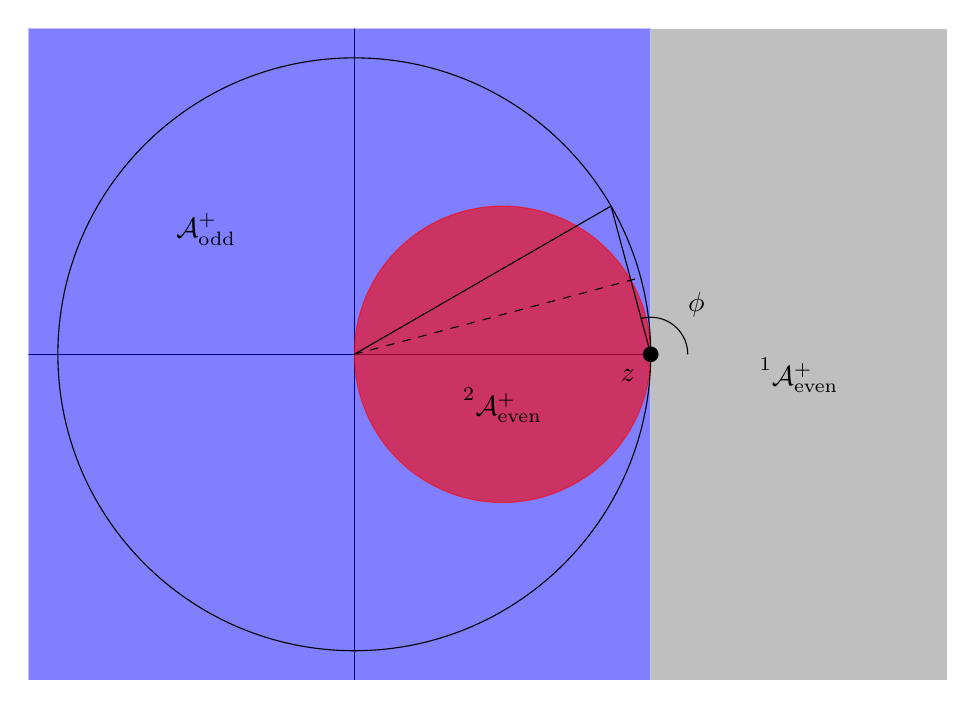
\begin{tikzpicture}
\begin{axis}[ 
    axis lines = middle,
    ticks = none,
    axis line style={-},
    ymin=-1.1, ymax=1.1,
    xmin=-1.1, xmax=2,
    axis equal image,
    height=4.5in
]
\draw[color=white, fill = lightgray] (axis cs:1, -1.1) rectangle (axis cs:2, 1.1);

\draw[color=white, fill = blue, opacity=0.5] (axis cs:-1.1, -1.1) rectangle (axis cs:1, 1.1);
\addplot[data cs=polar, red, opacity=0.6, domain=90:270,samples=180,smooth, fill=red, fill opacity=0.6] (x, {cos(x)});

\node[label={{$\prescript{1}{}{\aeven}$}}] at (axis cs:1.5,-0.2) {};
\node[label={{$\prescript{2}{}{\aeven}$}}] at (axis cs:0.5,-0.3) {};
\node[label={{$\aodd$}}] at (axis cs:-0.5,0.3) {};

\draw (axis cs:0,0) circle [radius=1];
\node[label={225:{$z$}},circle,fill,inner sep=2pt] at (axis cs:1,0) {};

\draw (axis cs:0,0) -- (axis cs:{cos(30)},{sin(30)});
\draw (axis cs:1,0) -- (axis cs:{cos(30)},{sin(30)});
\draw[dashed] (axis cs:0,0) -- (axis cs:{cos(15)},{sin(15)});

\draw (axis cs:1.125,0.0) arc(0:{90+15}:{transformdirectionx(0.125)}) (axis cs:{1-0.125},0);
\node[label={45:{$\phi$}}] at (axis cs:1.06,0.06) {};
\end{axis}
\end{tikzpicture}
\end{center}
Before jumping into calculations observe that we can parameterize our subset of $\mathbb{R}^5$ via $(\theta, r)$, as shown in the definition of the subsets above and put 
$$
s(\theta) = \begin{cases}
  -1 & \theta \in [\pi/2, 3\pi/2] \\
  1 & \textup{otherwise}
\end{cases}.
$$
We can simplify our integrand as follows:
\begin{IEEEeqnarray*}{rCl}
  J(r, \theta) &=& \frac{\parens{\bec{a} \cdot \bec{t}(z)} \bec{b} - \parens{\bec{b} \cdot \bec{t}(z)}\bec{a}}{r^{1+\sigma}} \\
  &=& \frac{
    \parens{\begin{pmatrix} \cos\theta \\ \sin\theta \end{pmatrix} \cdot \begin{pmatrix} 0 \\ 1 \end{pmatrix}}s(\theta) \begin{pmatrix} -\sin \theta \\ \cos \theta \end{pmatrix}
    - \parens{s(\theta)\begin{pmatrix} -\sin\theta \\ \cos\theta \end{pmatrix} \cdot \begin{pmatrix} 0 \\ 1 \end{pmatrix}}s(\theta) \begin{pmatrix} \cos \theta \\ \sin \theta \end{pmatrix}
    }{r^{1+\sigma}} \\
    &=& \frac{s(\theta) \parens{\sin\theta \begin{pmatrix} -\sin \theta \\ \cos \theta \end{pmatrix} - \cos\theta \begin{pmatrix} \cos \theta \\ \sin \theta \end{pmatrix}}}{r^{1+\sigma}} = \frac{-s(\theta) \begin{pmatrix} \sin^2\theta + \cos^2\theta \\ -\sin\theta\cos\theta + \cos\theta\sin\theta \end{pmatrix}}{r^{1+\sigma}} \\
      &=& \begin{pmatrix} -1 \\ 0 \end{pmatrix} \frac{s(\theta)}{r^{1+\sigma}}
\end{IEEEeqnarray*}
Next we can start computing integrals, we begin by integrating over $\aeven$:
\begin{IEEEeqnarray*}{rCl}
  \int_{\aeven} \frac{s(\theta)}{r^{1+\sigma}} \, d\mathcal{H}^2(r, \theta) &=& \parens{\int_{3\pi/2}^{2\pi} + \int_{0}^{\pi/2}} \int_\epsilon^\infty \frac{s(\theta)}{r^{1+\sigma}} \, dr \, d\theta + \int_{\pi/2}^{3\pi/2} \int_{\epsilon}^{\cos(\pi-\theta)} \frac{s(\theta)}{r^{1+\sigma}} \, dr \, d\theta \\
  &=& \parens{\int_{3\pi/2}^{2\pi} + \int_{0}^{\pi/2}} \int_\epsilon^\infty \frac{1}{r^{1+\sigma}} \, d r \, d\theta - \int_{\pi/2}^{3\pi/2} \int_{\epsilon}^{\cos(\pi-\theta)} \frac{1}{r^{1+\sigma}} \, dr \, d\theta \\
  &=& -\frac{1}{\sigma}\parens{\int_{3\pi/2}^{2\pi} + \int_{0}^{\pi/2}} \parens{ 0 - \frac{1}{\epsilon^\sigma} } \, d\theta + \frac{1}{\sigma} \int_{\pi/2}^{3\pi/2} \parens{\frac{1}{\parens{\cos(\pi-\theta)}^\sigma} - \frac{1}{\epsilon^\sigma}} \, d \theta \\
  &=& \frac{\pi}{\sigma\epsilon^\sigma} - \frac{\pi}{\sigma\epsilon^\sigma} - \frac{1}{\sigma} \int_{\pi/2}^{-\pi/2} \parens{\sec \theta}^\sigma \, d\theta \\
  &=& \frac{1}{\sigma} \int_{-\pi/2}^{\pi/2} \parens{\sec \theta}^\sigma \, d \theta.
\end{IEEEeqnarray*}
Now for $\aodd$:
\begin{IEEEeqnarray*}{rCl}
  \int_{\aodd} \frac{s(\theta)}{r^{1+\sigma}} \, d\mathcal{H}^2(r, \theta) &=& \int_{\pi/2}^{3\pi/2} \int_{\cos(\pi - \theta)}^\infty \frac{s(\theta)}{r^{1+\sigma}} \, dr \, d\theta \\
  &=& - \int_{\pi/2}^{3\pi/2} \int_{\cos(\pi - \theta)}^\infty \frac{1}{r^{1+\sigma}} \, dr \, d\theta \\
  &=& \frac{1}{\sigma} \int_{\pi/2}^{3\pi/2} \parens{0 - \frac{1}{\parens{\cos(\pi - \theta)}^\sigma}} \, d\theta \\
  &=& \frac{1}{\sigma}\int_{\pi/2}^{-\pi/2} \parens{\sec \theta}^\sigma \, d \theta \\
  &=& -\frac{1}{\sigma}\int_{-\pi/2}^{\pi/2} \parens{\sec \theta}^\sigma \, d\theta.
\end{IEEEeqnarray*}
Putting these computations together we have:
\begin{IEEEeqnarray*}{rl}
  \parens{\int_{\aeven} - \int_{\aodd}}& \frac{\parens{\bec{a} \cdot \bec{t}(z)} \bec{b} - \parens{\bec{b} \cdot \bec{t}(z)}\bec{a}}{r^{1+\sigma}} \, d\mathcal{H}^{2}\parens{\bec{a}, \bec{b}, r} \\
   &= \parens{\int_{\aeven} - \int_{\aodd}} \begin{pmatrix} -1 \\ 0 \end{pmatrix} \frac{s(\theta)}{r^{1+\sigma}} \, d\mathcal{H}^2 \\
   &= \begin{pmatrix} -1 \\ 0 \end{pmatrix} \parens{\frac{1}{\sigma} \int_{-\pi/2}^{\pi/2} \parens{\sec \theta}^\sigma \, d\theta + \frac{1}{\sigma} \int_{-\pi/2}^{\pi/2} \parens{\sec \theta}^\sigma \, d\theta} \\
   &= \begin{pmatrix} -1 \\ 0 \end{pmatrix} \frac{2}{\sigma} \int_{-\pi/2}^{\pi/2} \parens{\sec \theta}^\sigma \, d\theta \\
     &= \begin{pmatrix} -1 \\ 0 \end{pmatrix} \frac{2\sqrt{\pi}\gam{\frac{1-\sigma}{2}}}{\sigma\gam{1-\frac{\sigma}{2}}} \textup{ by \eqref{l2}}.
\end{IEEEeqnarray*}
Finally we can recover the classical curvature $\kappa = z''(0) = (-1, 0)$ as follows:
\begin{IEEEeqnarray*}{rCl}
  \lim_{\sigma \uparrow 1} \frac{\parens{1 - \sigma}}{4} \kappa_\sigma &=& \lim_{\sigma\uparrow 1} \begin{pmatrix} -1 \\ 0 \end{pmatrix} \frac{2\parens{1-\sigma}\sqrt{\pi} \gam{\frac{1-\sigma}{2}}}{4\sigma \gam{1-\frac{\sigma}{2}}} \\
    &=& \begin{pmatrix} -1 \\ 0 \end{pmatrix} \frac{\sqrt{\pi}}{2} \lim_{\sigma \uparrow 1} \frac{\parens{1-\sigma}\gam{\frac{1-\sigma}{2}}}{\sigma \gam{1 - \frac{\sigma}{2}}} \\
      &=& \begin{pmatrix} -1 \\ 0 \end{pmatrix} \frac{1}{2} \underbrace{\lim_{\sigma\uparrow 1} \parens{1-\sigma} \gam{\frac{1-\sigma}{2}}}_{\eqref{l3}} = \begin{pmatrix} -1 \\ 0 \end{pmatrix} = \kappa.
\end{IEEEeqnarray*}

\subsection{Definitions \& Properties}
For the sake of completeness we use the following definitions are used:
\begin{IEEEeqnarray}{rCl}
  \gam{z} &=& \int_0^\infty t^{z-1} e^{-t} \, dt \textup{ where } \Re(z) > 0, \label{d1} \\
  \bet{z_1, z_2} &=& \int_0^1 t^{z_1 - 1} \parens{1-t}^{z_2-1} \, dt \textup{ where } \Re(z_1), \Re(z_2) > 0. \label{d2}
\end{IEEEeqnarray}
And we will assume the following properties:
\begin{IEEEeqnarray}{rCl}
  \bet{z_1, z_2} &=& \frac{\gam{z_1}\gam{z_2}}{\gam{z_1+z_2}}, \label{p1} \\
  \gam{z}\gam{1-z} &=& \frac{\pi}{\sin \parens{\pi z}}. \label{p2}
\end{IEEEeqnarray}
The former can be shown via a direct computation of the product $\gam{z_1}\gam{z_2}$ and change of variables \& the latter via Weierstrass products.
\newpage
\subsection{Calculations}
\begin{lemma}\label{l1}
  $$
  \gam{\frac{1}{2}} = \sqrt{\pi}
  $$
\end{lemma}
\begin{proof}
  From \eqref{p2} we have:
  $$
  \parens{\gam{\frac{1}{2}}}^2 = \gam{\frac{1}{2}} \gam{\frac{1}{2}} = \frac{\pi}{\sin\parens{\frac{\pi}{2}}} = \pi.
  $$
\end{proof}
\begin{lemma}\label{l2}
  $$
  \int_{-\pi/2}^{\pi/2} \parens{\cos\theta}^{-\sigma} \, d \theta = \frac{\sqrt{\pi}\gam{\frac{1-\sigma}{2}}}{\gam{1-\frac{\sigma}{2}}} \textup{ for } \sigma \in (0, 1)
  $$
\end{lemma}
\begin{proof}
  Beginning with \eqref{d2} and using a change of variables $t \to \sin^2 \theta$ so that $1 - t = \cos^2 \theta$ and $dt = 2\sin\theta \cos\theta \, d\theta$, thus
  $$
  \bet{z_1, z_2} = \int_0^{\pi/2} \parens{\sin \theta}^{2z_1 - 2} \parens{\cos \theta}^{2z_2 - 2} \cdot 2 \sin\theta\cos\theta \, d\theta = 2\int_0^{\pi/2} \parens{\sin \theta}^{2z_1-1} \parens{\cos\theta}^{2z_2 - 1} \, d\theta.
  $$
  Now, since $\frac{1-\sigma}{2} > 0$ when $\sigma < 1$ we have:
  $$
  \bet{\frac{1}{2}, \frac{1-\sigma}{2}} = 2\int_0^{\pi/2} \parens{\sin \theta}^{0} \parens{\cos\theta}^{1 - \sigma - 1} \, d\theta = 2\int_0^{\pi/2} \parens{\cos\theta}^{-\sigma} \, d\theta = \int_{-\pi/2}^{\pi/2} \parens{\cos\theta}^{-\sigma} \, d\theta.
  $$
  Notice the final equality comes from the fact that $\cos\theta$ is even. On the other hand, by \eqref{p1} we know
  $$
  \bet{\frac{1}{2}, \frac{1-\sigma}{2}} = \frac{\gam{1/2}\gam{\frac{1-\sigma}{2}}}{\gam{\frac{1}{2} + \frac{1-\sigma}{2}}}.
  $$
  Leveraging \eqref{l1} we find our desired equality.
\end{proof}
\begin{lemma}\label{l3}
  $$
  \lim_{\sigma\uparrow 1} \parens{1-\sigma} \gam{\frac{1-\sigma}{2}} = 2.
  $$
\end{lemma}
\begin{proof}
  By \eqref{p2} we know
  $$
  \gam{\frac{1-\sigma}{2}} = \frac{\pi}{\sin\parens{\pi \frac{1-\sigma}{2}}} \cdot \frac{1}{\gam{\frac{1+\sigma}{2}}}.
  $$
  Thus we have
  \begin{IEEEeqnarray*}{rCl}
    \lim_{\sigma\uparrow 1} \parens{1-\sigma} \gam{\frac{1-\sigma}{2}} &=& \lim_{\sigma \uparrow 1} \frac{\parens{1-\sigma}\pi}{\sin\parens{\pi \frac{1-\sigma}{2}}} \cdot \frac{1}{\gam{\frac{1+\sigma}{2}}} = \parens{\lim_{\sigma \uparrow 1} \frac{\parens{1-\sigma}\pi}{\sin\parens{\pi \frac{1-\sigma}{2}}}} \cdot \parens{\lim_{\sigma\uparrow 1} \frac{1}{\gam{\frac{1+\sigma}{2}}}} \\
    &=& \pi \lim_{\sigma \uparrow 1} \frac{\parens{1-\sigma}}{\sin\parens{\pi \frac{1-\sigma}{2}}} \underbrace{= \pi \lim_{\sigma\uparrow 1} \frac{-1}{\cos\parens{\pi\frac{1-\sigma}{2}}\cdot \frac{-\pi}{2}}}_{\text{L'Hôpital's rule}} = 2
  \end{IEEEeqnarray*}
\end{proof}
\end{document}
